En resumen, en nuestra prueba de calibración de los SiPM tenemos una caja que actuará como jaula de Faraday, con temperatura y humedad controlada y apantallada en lo posible de la luz del exterior. 

En su interior colocamos un diodo LED que emite fotones de $\lambda=435~\nm$, un SiPM, que emite un impulso de intensidad cada vez que detecte uno o más  fotones  y una tarjeta que convierte este impulso de intensidad en un impulso de voltaje. Finalmente llevamos este impulso de voltaje a un osciloscopio (marca TELEDYNE LECROY, modelo WwaveRunner 625Zi) que lo analiza. 
Una vez en el osciloscopio, la señal que recibimos cuando se enciende el diodo LED es similar a la de la señal superior de la figura~\ref{analisis} (amarilla)~\cite{inftec}. Para el análisis,  se  activa el modo persistencia del osciloscopio con el objetivo de comparar señales de distintas alturas. Estas señales corresponden a distinto número de pixels activados en cada instante de tiempo ya que, como hemos dicho anteriormente, la señal de salida del sistema es la suma de las señales de los pixeles activados. La señal se muestra superpuesta a la señal de sincronización del generador de señales (verde) que nos muestra cuando se ha encendido el diodo LED y que, por tanto, actúa como trigger.

El objetivo ahora es calcular la ganancia del sistema. Dado que únicamente existen dos ganancias en el sistema (SiPM y tarjeta) y conocemos la ganancia de la tarjeta, mencionada en la sección anterior, determinando la ganancia total podremos determinar de forma aproximada la ganancia del SiPM. 

\begin{equation}
G_{tot}=G_{SiPM} \cdotp G_{card} \longrightarrow G_{SiPM} = \frac{G_{tot}}{G_{card}}
\label{ganancias}
\end{equation}

Para medir la ganancia total realizamos una integral del área de cada uno de los impulsos de salida del sistema y guardamos el resultado en un histograma. De esta forma, obtenemos un histograma de las cargas de los pulsos. La ventana temporal sobre la que se integra es aproximadamente una división, que equivale a $500~\ns$. Esta se ajusta con bastante precisión al impulso, algo muy importante para evitar la introducción de fondo.

Dado que idealmente el impulso producido por  los pixel son idénticos, el histograma obtenido debería ser  un conjunto deltas de Dirac equiespaciadas. Sin embargo, hay que tener en cuenta que la cascada que produce cada uno de estos fotones detectados en cada pixel esta sometido a fluctuaciones estadísticas. Además, los propios instrumentos de medidas empleados tienen una incertidumbre inherente. Hay que tener en cuenta que también tenemos distintas fuentes de fondo, como la corriente oscura (ruido térmico), fotones de luz del exterior, etc. 
Como resultado de todo esto, lo que obtenemos un conjunto de gaussianas equiespaciadas. En la figura~\ref{analisis} inferior puede verse el resultado de una toma de datos de $25000$ eventos a $25~\celsius$, $60\%$ de humedad y $V_{ov}=3~\volt$,

\begin{figure}[hbtp]
 \centering
 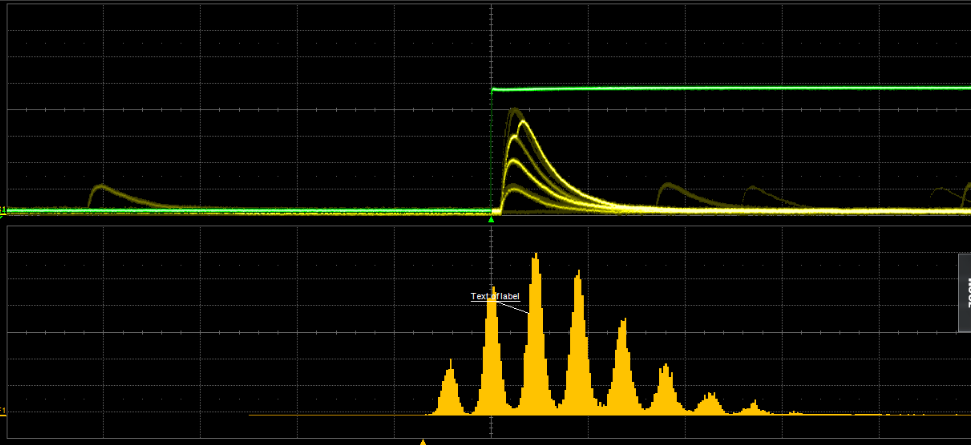
\includegraphics[scale=0.4]{Analisis.png}
 \caption{Análisis\label{analisis}}
 \end{figure}
donde cada uno de los picos corresponde a la carga de un número de pixels activados (uno, dos, etc.). El primer pico no debe tenerse en cuenta en el análisis, ya que este corresponde al pedestal (cero pixels activados). Su origen es debido a la existencia de las cuentas oscuras.
 
Hemos desarrollado una macro en ROOT$~\cite{manualROOT}$ que, utilizando la librería TSpectrum (especialmente diseñada para el análisis de histogramas con picos) para obtener la ganancia del sistema. Su diagrama de flujo es el siguiente:
\begin{enumerate}
\item {} Primero la macro lee el fichero de datos, los guarda en una variable de tipo histograma y los representa. La macro termina de leer el fichero cuando no encuentra más valores.

\item {} A continuación, a partir de una función de la librería TSpectrum, busca en este histograma y devuelve el número de gausianas que ha encontrado y su posición.

\item {} Seguidamente ajusta todos los datos del histograma a una recta y solo se queda con las gausianas, cuya norma sobrepasa en altura a esta recta. El objetivo de este paso es que, en casos muy concretos (temperatura alta o luz del laboratorio encendida) tenemos mucho ruido y, aparece un fondo,  que el programa ajusta a una gausiana y, como consecuencia calcula la ganancia de manera incorrecta. Un ejemplo de este caso se muestra en la figura$~\ref{fondogrande}$.

\begin{figure}[hbtp]
\centering
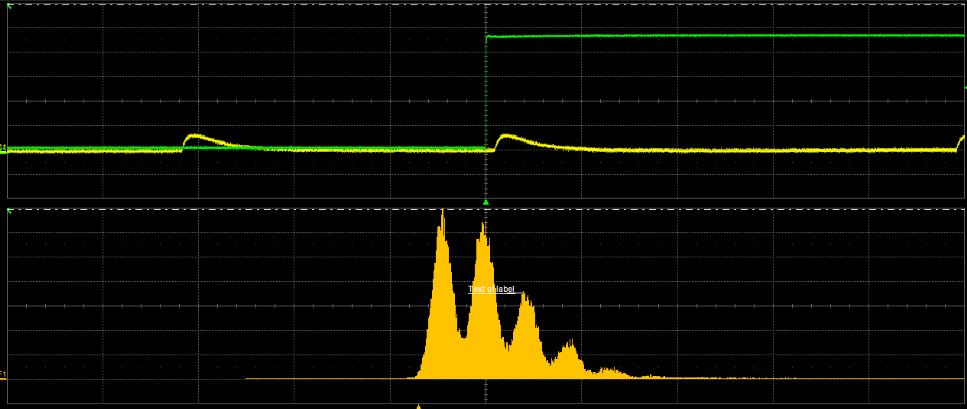
\includegraphics[scale=0.4]{fondogaussiano.png}
\caption{Espectro con mucho fondo\label{fondogrande}}
\end{figure}

\item {} A continuación, ajustamos el espectro a una recta más una suma de $n$ gausianas, donde $n$ es el número de gausianas que superan la recta (calculado en el paso anterior). La necesidad de utilizar una recta es debido a que siempre vamos a tener corriente oscura y otro tipo de fondo que aparecen como una linea base en el histograma, como puede verse en la figura~\ref{analisis}. Podemos apreciar en la figura~\ref{Root} que el ajuste (linea roja) es relativamente bueno. Para determinar si ajuste es aceptable aplicamos el test $\chi^2$. En este caso se obtuvo un resultado de $\frac{\chi^2}{ndf}=\frac{1276}{223}\approx 5.72$. Vemos que efectivamente, el ajuste lineal representa bien los datos.

\begin{figure}[hbtp]
\centering
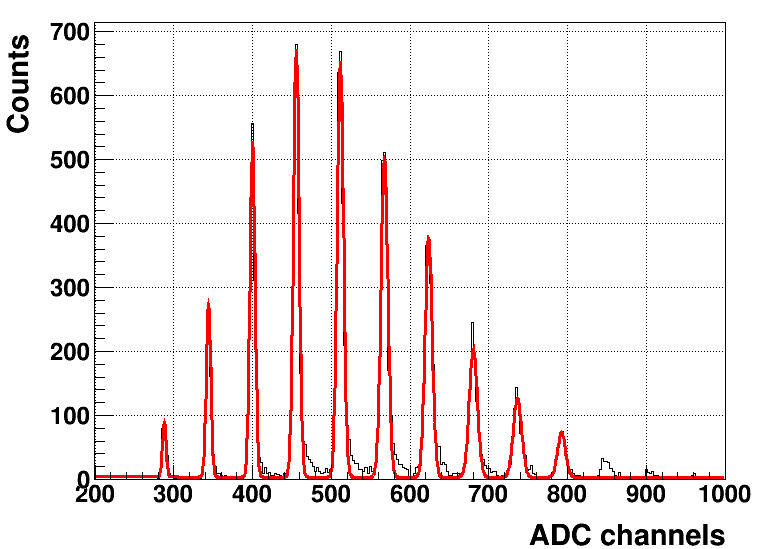
\includegraphics[scale=0.4]{AjusteEspectro1.png}
\caption{ Ajuste de la macro de ROOT sobre un espectro\label{Root}}
\end{figure}

\item {} Dado que se ha observado que, aun con el tercer paso, existen situaciones límites en que el fondo sigue superando la recta, se ha incluido un paso en la macro en la cual se acepta por teclado uno a uno los picos que serán utilizados en el análisis. Además, la macro calcula la resolución de cada gaussiana y la resolución total, obtenida a partir de la suma cuadrática de la resolución de cada gaussiana. Los valores habitualmente encontrados en los análisis se encuentran en el intervalo $1.5\% - 5\%$, valores bastante aceptables.

\item {} Finalmente, la macro ordena los picos según su posición en el espectro y calcula la ganancia por dos caminos:
	\begin{enumerate}

	\item {} Por un lado se ha calculado la distancia promedio entre sucesivas gausianas del espectro~\cite{Hueso}.
	\begin{equation} 
	Q = G N_\gamma + Q_0 \longrightarrow \Delta Q= Q_{N_\gamma} - Q_{N_\gamma -1}=G N_\gamma+ Q_0 - G(N_		\gamma -1) - Q_0 = G
	\label{gananciametodo1}
	\end{equation}
	Podemos observar que este cálculo corresponde a la ganancia. Hay que tener en cuenta que se han empleado factores de conversión para convertir la posición del pico (inicialmente en unidades de	tensión $\volt$) en unidades de carga $\coulomb$. En concreto, se ha utilizado el factor $\frac{1}{eR}$, donde $R$ es la resistencia del osciloscopio, $50~\ohm$ y $e$ es la carga del electrón.
	
	\item {} Por otro lado, se ha ajustado a una recta las posiciones horizontales de estas gausianas en el 	espectro frente a el número de píxeles. Esto nos da la siguiente ecuación~\cite{Hueso}:
	\begin{equation}
	Centro\_pico(V) = GeRN_\gamma + k_0
	\label{gananciametodo2}
	\end{equation}
	 Vemos por tanto, que a partir del valor de la pendiente podemos obtener	el valor de la ganancia. La figura~\ref{ajuste} muestra un ejemplo de ajuste de posiciones de gausianas y número de píxeles para el caso de $25~\celsius$, humedad de $45\%$ y $V_{ov}=3~\volt$. Podemos observar que existe	un acuerdo excelente, algo que ocurre prácticamente en la totalidad de los casos. Las barras de error  de este gráfico  no son apreciables en esta  escala.
		
	\begin{figure}[hbtp]
		\centering
		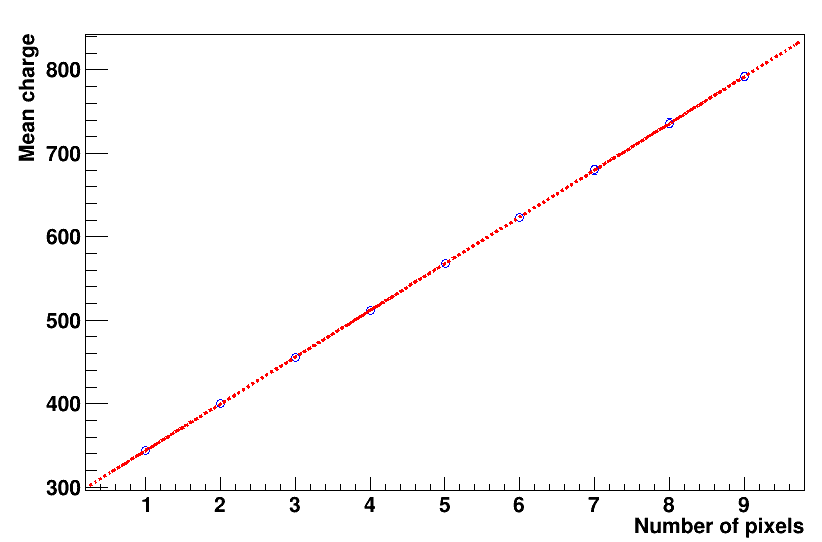
\includegraphics[scale=0.4]{FitPosicionPixels.png}
		\caption{Ajuste carga de las señales del SiPM frente al número de píxeles encendidos\label{ajuste}}
		\end{figure}
			
	\end{enumerate}
	
Para este caso concreto las ganancias obtenidas por los dos caminos anteriores son respectivamentente:
\begin{equation}
G_1= 6.38938 \cdot 10^8 \pm 2.15953 \cdot 10^8
\label{gananciatotalmetodo1} 
\end{equation}
\begin{equation}
G_2=7.18235 \cdot 10^8 \pm 6.88392 \cdot 10^6
\label{gananciatotalmetodo2}
\end{equation}
Por extensión, las ganancias del SiPM calculadas por cada camino son (aproximadamente)$\eqref{ganancias}$: 
\begin{equation}
G_1= 5.80853 \cdot 10^6 \pm 1.96321 \cdot 10^6
\label{gananciaSiPMmetodo1}
\end{equation}
\begin{equation}
G_2= 6.52941 \cdot 10^6 \pm 6.258 \cdot 10^4
\label{gananciaSiPMmetodo2}
\end{equation}
donde los errores se han obtenido por propagación. Si comparamos con la bibliografía~\cite{datasheet SiPM} podemos observar que ambos valores son bastante aceptables, con errores relativos de:

\begin{equation}
\sigma_{rel1} \approx 0.0319 = 3.19\%; \qquad \sigma_{rel2} \approx 0.0882 = 8.82\%
\label{erroresgananciasSiPM}
\end{equation}


Dado que, en la práctica, las gausianas no están perfectamente equiespaciadas debido a errores e incertidumbres, consideraremos como más fiable el segundo método, ya que se trata de un método más formal, a pesar de tener un error relativo mayor.
El test $\chi^2$ da un valor de  $\frac{\chi^2}{ndf}=\frac{0.05452}{7}\approx 0.008$, bastante inferior a la unidad, debido  probablemente a que se han sobreestimado los errores de las medidas (calculados a partir de las desviaciones típicas de las gausianas del ajuste de la figura $\ref{Root}$).

\end{enumerate}